\documentclass{ximera}
\input{../preamble.tex}

\title{Exercises} \license{CC BY-NC-SA 4.0}

\begin{document}

\begin{abstract}
\end{abstract}
\maketitle

\begin{onlineOnly}
\section*{Exercises}
\end{onlineOnly}


\begin{problem}\label{exer:6.4.1}
Find the equation of the curve
\begin{equation}\label{eq:eqA6.4.1}
r=\frac{\rho}{1+e\cos(\theta-\phi)}
\end{equation}
in terms of
$(X,Y)=\left(r\cos(\theta-\phi),r\sin(\theta-\phi)\right)$,
which are rectangular coordinates with respect to the axes shown in the
figure below. %~\ref{figure:6.4.5}. 
Use your results to verify that
\ref{eq:eqA6.4.1}
is the equation of an ellipse if $0<e<1$, a parabola if $e=1$,
or a hyperbola if $e>1$. If $e<1$, leave your answer in
the form
$$
 \frac{(X-X_0)^2}{a^2}+\frac{(Y-Y_0)^2}{b^2}=1,
$$
and show that the area of the ellipse is
$$
A=\frac{\pi\rho^2}{(1-e^2)^{3/2}}.
$$
Then use Theorem~\ref{thmtype:6.4.1} to show that the time required for
the object to traverse the entire orbit is
$$
T=\frac{2\pi\rho^2}{h(1-e^2)^{3/2}}.
$$
(This is
\href{http://www-history.mcs.st-and.ac.uk/Mathematicians/Kepler.html}
{Kepler's third law};   $T$ is called the
\emph{period} of the orbit.)

\begin{center}
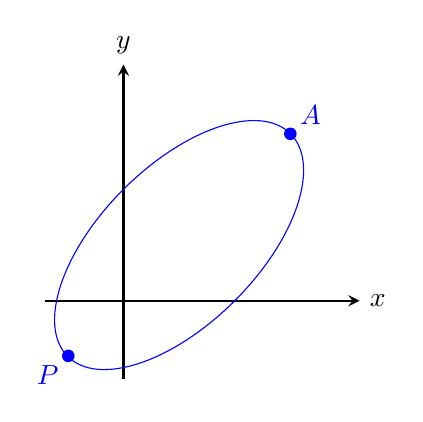
\begin{tikzpicture}[scale=2]
 \draw[-stealth, thick] (0,-0.5) -- (0,1.5) node[above] {$y$};
 \draw[-stealth, thick] (-0.5,0) -- (1.5,0) node[right] {$x$};
\draw[blue,rotate=45] (0.5,0) ellipse (1 and 0.5);
 \fill[blue] (-0.35,-0.35)node[below left]{$P$} circle (0.04);
\fill[blue] (1.06,1.06)node[above right]{$A$} circle (0.04);
\end{tikzpicture}
\end{center}

%\begin{image}
 % \includegraphics[height=1.5in]{fig060405.jpg}
%\end{image}
\end{problem}

\begin{problem}\label{exer:6.4.2}
Suppose an object with mass $m$ moves in the $xy$-plane under the
central force
$$
{\bf F}(r,\theta)=-\frac{mk}{r^2}(\cos\theta\,{\bf i}+\sin\theta\,{\bf
j}),
$$
where $k$ is a positive constant. As we shown, the orbit of the
object is given by
$$
r=\frac{\rho}{1+e\cos(\theta-\phi)}.
$$
Determine $\rho$, $e$, and $\phi$ in terms of the initial conditions
$$
r(0)=r_0,\quad  r'(0)=r_0', \text{\; and \;} \theta(0)=\theta_0,\quad
\theta'(0)=\theta_0'.
$$
Assume that the initial position and velocity vectors are not
collinear.

\begin{solution}
    Let $h=r_0^2\theta_0'$; then $\rho=\frac{h^2}{ k}$. Since
$r=\frac{\rho}{ 1+e\cos(\theta-\phi)}$, it follows that (A)
$e\cos(\theta-\phi)=\frac{\rho}{ r}-1$. Differentiating this with
respect to $t$ yields $-e\sin(\theta-\phi)\theta'=-\frac{\rho r'}{
r^2}$, so (B) $e\sin(\theta-\phi)=\frac{\rho r'}{ h}$, since
$r^2\theta'\equiv h$.
Squaring and adding (A) and (B) and setting $t=0$ in the result yields
$e=\left[\left(\frac{\rho}{ r_0}-1\right)^2+\left(\frac{\rho r_0'}{
h}\right)^2\right]^{1/2}$. If $e=0$, then $\theta_0$ is undefined, but
also irrelevant; if $e\ne0$, then set $t=0$ in (A) and (B) to see that
$\phi=\theta_0-\alpha$, where $-\pi\le\alpha<\pi$,
$\cos\alpha=\frac{1}{ e}\left(\frac{\rho}{ r_0}-1\right)$ and
$\sin\alpha=\frac{\rho r_0'}{ eh}$

\end{solution}
\end{problem}

\begin{problem}\label{exer:6.4.3}
Suppose we wish to put a satellite with mass $m$ into an
elliptical orbit around Earth. Assume that the only force acting on
the object is Earth's gravity, given by
$$
{\bf F}(r,\theta)=-mg\left(\frac{R^2}{r^2}\right)(\cos\theta\,{\bf
i}+\sin\theta\,{\bf j}),
$$
where $R$ is Earth's radius, $g$ is the acceleration due to gravity at
Earth's surface, and $r$ and $\theta$ are polar coordinates in the
plane of the orbit, with the origin at Earth's center.

\begin{enumerate}
\item % (a)
Find the eccentricity required to make the aphelion and perihelion
distances equal to $R\gamma_1$ and $R\gamma_2$, respectively, where
$1<\gamma_1<\gamma_2$.
\item % (b)
Find the  initial conditions
$$
r(0)=r_0,\quad  r'(0)=r_0', \text{\; and \;} \theta(0)=\theta_0,\quad
\theta'(0)=\theta_0'
$$
required to make the initial point the perigee, and the motion along
the orbit in the direction of increasing $\theta$. 
\begin{hint}
    Use the
results of Exercise~\ref{exer:6.4.2}.
\end{hint}
\end{enumerate}
\end{problem}

\begin{problem}\label{exer:6.4.4}
 An object with mass $m$  moves in a spiral orbit
$r=c\theta^2$ under a central force
$$
{\bf
F}(r,\theta)=f(r)(\cos\theta\,{\bf i}+\sin\theta\,{\bf j}).
$$
Find $f$.

\begin{solution}
    Recall that
(A) $\frac{d^{2}u}d{\theta^{2}}=-\frac{1}{mh^{2}u^{2}}f(1/u)$.
Let $u=\frac{1}{ r}=\frac{1}{ c\theta^2}$; then $\frac{d^2u}{
d\theta^2}=\frac{6}{ c\theta^4}= 6cu^2$.
 $6cu^2+u=-\frac{1}{ mh^2u^2}f(1/u)$, so
$f(1/u)=-mh^2(6cu^4+u^3)$ and $f(r)=-mh^2\left(\frac{6c}{
r^4}+\frac{1}{ r^3}\right)$.
\end{solution}
\end{problem}

\begin{problem}\label{exer:6.4.5}
 An object with mass $m$  moves in the orbit
$r=r_0e^{\gamma\theta}$ under a central force
$$
 {\bf
F}(r,\theta)=f(r)(\cos\theta\,{\bf i}+\sin\theta\,{\bf j}).
$$
 Find $f$.
\end{problem}

\begin{problem}\label{exer:6.4.6}
Suppose an object with mass $m$ moves under the central force
$$
{\bf F}(r,\theta)=-\frac{mk}{r^3}(\cos\theta\,{\bf i}+\sin\theta\,{\bf
j}),
$$
with
$$
r(0)=r_0,\quad  r'(0)=r_0', \text{\; and \;} \theta(0)=\theta_0,\quad
\theta'(0)=\theta_0',
$$
 where $h=r_0^2\theta_0'\ne0$.
\begin{enumerate}
\item % (a)
 Set up a second order initial
value problem for $u=1/r$ as a function of~$\theta$.
\item % (b)
Determine $r=r(\theta)$ if (i) $h^2<k$;\;   (ii) $h^2=k$;\;   (iii)
$h^2>k$.
\end{enumerate}

\begin{solution}
\begin{enumerate}
    \item With $f(r)=-\frac{mk}{ r^3}$, Eqn.~6.4.11 becomes
(A) $\frac{d^2u}{ d\theta^2}+\left(1-\frac{k}{ h^2}\right)u=0$. The
initial conditions imply that $u(\theta_0)=\frac{1}{ r_0}$ and
$\frac{du}{ d\theta}(\theta_0)=-\frac{r_0'}{ h}$ (see
Eqn.~(6.4.)

\item Let $\gamma=\left|1-\frac{k}{ h^2}\right|^{1/2}$. (i) If
$h^2<k$, then (A) becomes $\frac{d^2u}{ d\theta^2}-\gamma^2u=0$, and
the solution of the initial value problem for $u$ is $u=\frac{1}{
r_0}\cosh\gamma(\theta-\theta_0)-\frac{r_0'}{\gamma
h}\sinh\gamma(\theta-\theta_0)$; therefore $r=r_0\left(
\cosh\gamma(\theta-\theta_0)-\frac{r_0r_0'}{\gamma
h}\sinh\gamma(\theta-\theta_0)\right)^{-1}$. (ii) If $h^2=k$, then (A)
becomes $\frac{d^2u}{ d\theta^2}=0$, and the solution of the initial
value problem for $u$ is $u=\frac{1}{ r_0}-\frac{r_0'}{
h}(\theta-\theta_0)$; therefore $r=r_0\left(1 -\frac{r_0r_0'}{
h}(\theta-\theta_0)\right)^{-1}$. (iii) If $h^2>k$, then (A) becomes
$\frac{d^2u}{ d\theta^2}+\gamma^2u=0$, and the solution of the
initial value problem for $u$ is $u=\frac{1}{
r_0}\cos\gamma(\theta-\theta_0)-\frac{r_0'}{\gamma
h}\sin\gamma(\theta-\theta_0)$; therefore $r=r_0\left(
\cos\gamma(\theta-\theta_0)-\frac{r_0r_0'}{\gamma
h}\sin\gamma(\theta-\theta_0)\right)^{-1}$.
\end{enumerate}
\end{solution}
\end{problem}



\end{document}